\section{DIAGRAMA DE CASOS DE USO}

De acordo com \citeonline{umlGuiaDoUsuario}, um caso de uso especifica o
comportamento essencial de um sistema ou subsistema em uma visão macro, sem que
haja a implementação de tal funcionalidade, permitindo que, desenvolvedores, 
usuários e especialistas do domínio de negócio possam compreender as ações e 
papéis envolvidos no sistema, além disto, serve para a validação da arquitetura 
e da aplicação (ao decorrer da implementação do projeto de software). Na Figura
\ref{fig:diagramaCasosDeUso}, é apresentado diagrama de casos de uso da aplicação.

\begin{figure}[h!tb]
	\caption{Diagrama UML de Casos de Uso}
	\label{fig:diagramaCasosDeUso}

	\centering
	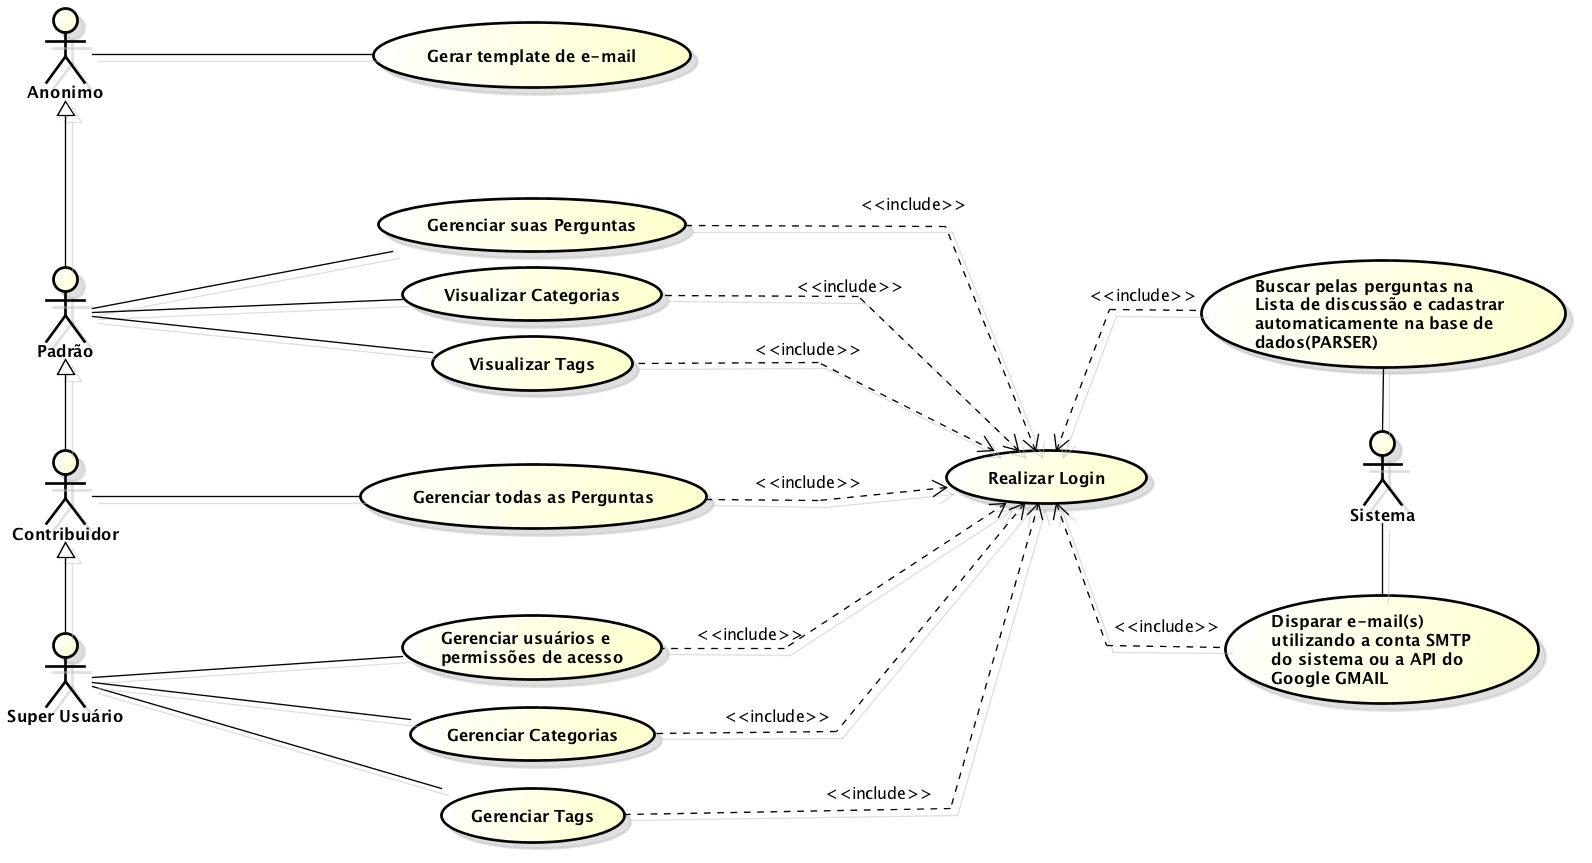
\includegraphics[width=\textwidth]{images/usecase.png}

	\centering
	\footnotesize Fonte: \fonteOAutor
\end{figure}

\FloatBarrier 	% Este comando impede que as imagens
				% flutuem a partir deste ponto no seu documento

O diagrama de casos de uso apresentado na Figura \ref{fig:diagramaCasosDeUso}
evidencia que todos os processos (exceto a geração do template de e-mail) só
podem ser realizados caso o usuário esteja autenticado na ferramenta.